\section{Experiment}
\label{kap:5}

V predošlých kapitolách sme podrobne preskúmali niekoľko rozdielnych prístupov k riešeniu nášho problému. Každý z týchto prístupov má svoje vlastné výhody a nevýhody, ktoré sme v práci analyzovali. V tejto kapitole sa však presunieme k ďalšiemu kroku nášho výskumu, ktorým je experimentálne porovnanie týchto prístupov.

Cieľom tejto kapitoly je zhromaždiť dáta a výsledky z experimentov, ktoré sme uskutočnili na každom z prístupov. Budeme sa venovať sledovaniu viacerých aspektov, ako je čas výpočtu, úspešnosť nájdenia trajektórie a kvalita výslednej trajektórie.

Našim hlavným záujmom je identifikovať najefektívnejší a najpresnejší prístup pre našu konkrétnu úlohu. Tento proces bude zahŕňať vyhodnotenie a porovnanie výsledkov každého prístupu vzhľadom na jeho schopnosť dosiahnuť požadovaný cieľ.

Na základe získaných údajov budeme schopní poskytnúť podrobnú analýzu týkajúcu sa vhodného prístupu k plánovaniu trajektórie pre našu konkrétnu úlohu.

\subsection{Opis experimentu}

Aby sme mohli spoľahlivo porovnať a vyhodnotiť schopnosti jednotlivých prístupov, je nevyhnutné, aby sme všetky testy vykonávali na rovnakých dátach a pri rovnakých podmienkach. Pre náš experiment sme preto vygenerovali štandardizovanú databázu vstupov, ktoré budeme následne používať pri vyhodnocovaní každého prístupu zvlášť. Týmto spôsobom zabezpečíme, že každý test bude založený na rovnakých podmienkach a budeme schopní presne porovnať ich výsledky a úspešnosť.

Databáza vstupov by sme si vedeli v jednoduchosti predstaviť ako veľké množstvo objektov rôznych veľkostí náhodne umiestnených v krabici. Každý objekt je definovaný rozmermi - výška, šírka, pozíciou a orientáciou. Veľkosť generovaných objektov sme si stanovali na základe rozmerov krabice, v ktorej sú objekty v sklade umiestnené. Rozmery krabice sú $ 460x745 mm $. Rozmery objektov sme generovali od veľkosti $ 100x200 mm $ po $ 400x600 mm $  a  zväčšovali sme ich po $ 20mm $. 

Snažíme sa nájsť hraničné situácie každého z algoritmov a preto sme si kontrolovali veľkosť uhlopriečky objektu. Ak bola uhlopriečka menšia ako $ 370 mm $, daný rozmer sa preskočil.  

Pre každú kombináciu rozmerov bola krabica rozdelená na 9 častí, pričom v každej z danej pozícii sme daný objekt rotovali s posunom $ 9 \degree $. Každá z daných pozícií bola kontrolovaná na kolíziu aby neboli generované nereálne konfigurácie. Takýmto spôsobom sme vygenerovali  11 440 vstupov, na ktorých bol následne každý z algoritmov testovaný. 

Testovanie prebiehalo načítaním dát z predom pripravenej databázy vstupov. Pre každú konfiguráciu sme spustili vybraný algoritmus a zaznamenali výstupné dáta, na základe ktorých sme následne porovnali jednotlivé prístupy. Výstupné dáta zahŕňali informácie o tom, či bolo úspešne nájdené spojenie medzi počiatočným a cieľovým bodom, čas potrebný na výpočet algoritmu a v prípade využitia predrotácie, aj jej hodnotu. Okrem toho sme zaznamenávali aj výslednú trajektóriu, ktorú tvorili jednotlivé prejazdové body. Takto získané dáta nám poslúžia na dôkladné porovnanie výkonnosti a účinnosti jednotlivých algoritmov.

Na porovnanie jednotlivých algoritmov plánovania z hľadiska kvality trajektórie sme si vypočítali pomer medzi priamou cestou z počiatku do cieľa a vzdialenosti danej cesty. Pri počítaní priamej cesty sme neuvažovali kolízie, ide o najkratšiu cestu v priestore, na ktorej výpočet sme v kartézskom súradnicovom systéme použili euklidovskú vzdialenosť a pri kĺbovom súradnicovom systéme sumu rozdielov medzi uhlami natočenia jednotlivých kĺbov medzi počiatočnou a cieľovou konfiguráciou.  

\subsection{3 stupne voľnosti}
\label{kap:5.1}
Kinematickú štruktúru s tromi stupňami voľnosti sme testovali pre plánovanie v kartézskom aj kĺbovom priestore. 

\subsubsection{Kartézsky priestor - RRT}

Najzákladnejším riešením bolo použitie jednoduchého RRT algoritmu v kartézskom priestore. Celková úspešnosť na testovacím dátach dosiahla $ 89,14 \% $. Na obrázku \ref{OBRAZOK 5.1.1} môžeme vidieť graf, ktorý nám ukazuje priemernú úspešnosť pre jednotlivé kombinácie rozmerov objektu. Na osi $ x $ sa nachádza šírka objektu, na osi $ y $ výška. Úspešnosť nájdenia riešenia je v jednotlivých bodoch vyjadrená farbou. Ako môžeme vidieť na škále vedľa grafu - Zelená farba nám predstavuje maximálnu úspešnosť a červená farba minimálnu.
\begin{figure}[h!]
	\centering
	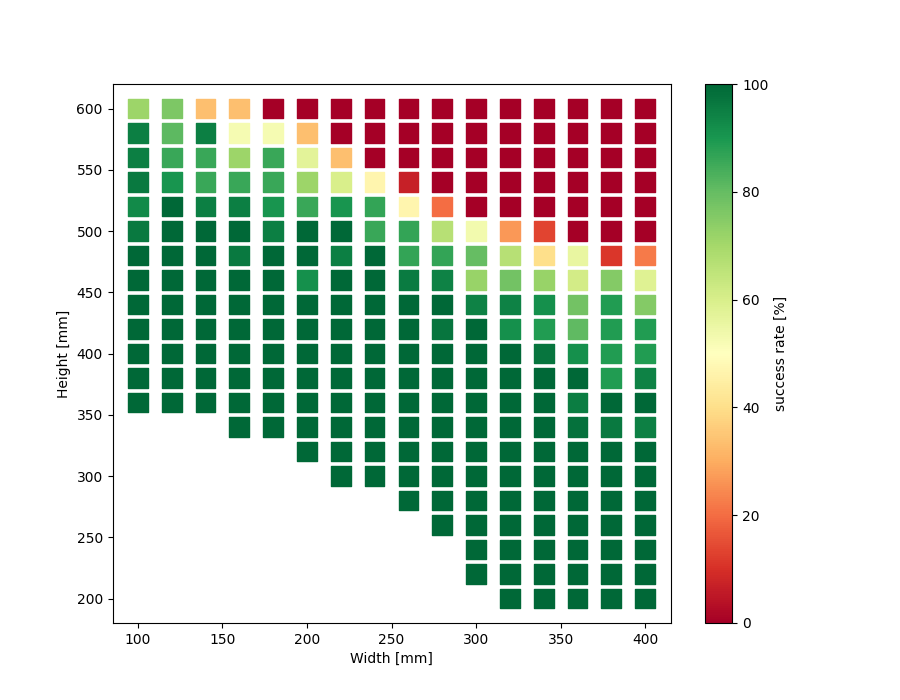
\includegraphics[width=140mm]{img/XYA-size.png}
	\caption{Kartézsky priestor (RRT) - úspešnosť } \label{OBRAZOK 5.1.1} 
\end{figure} 

Maximálny rozmer prenášaného objektu pri tomto algoritme by sme mohli určiť priamkou prechádzajúcou grafom bodmi - $ 100x580  $a $ 400x380 $. Na obrázku \ref{OBRAZOK 5.1.2} môžeme vidieť vizualizáciu rozmerov v pracovnom priestore robota.  
\begin{figure}[h]
	\centering
	\begin{subfigure}{0.4\textwidth}
		\centering
		\fbox{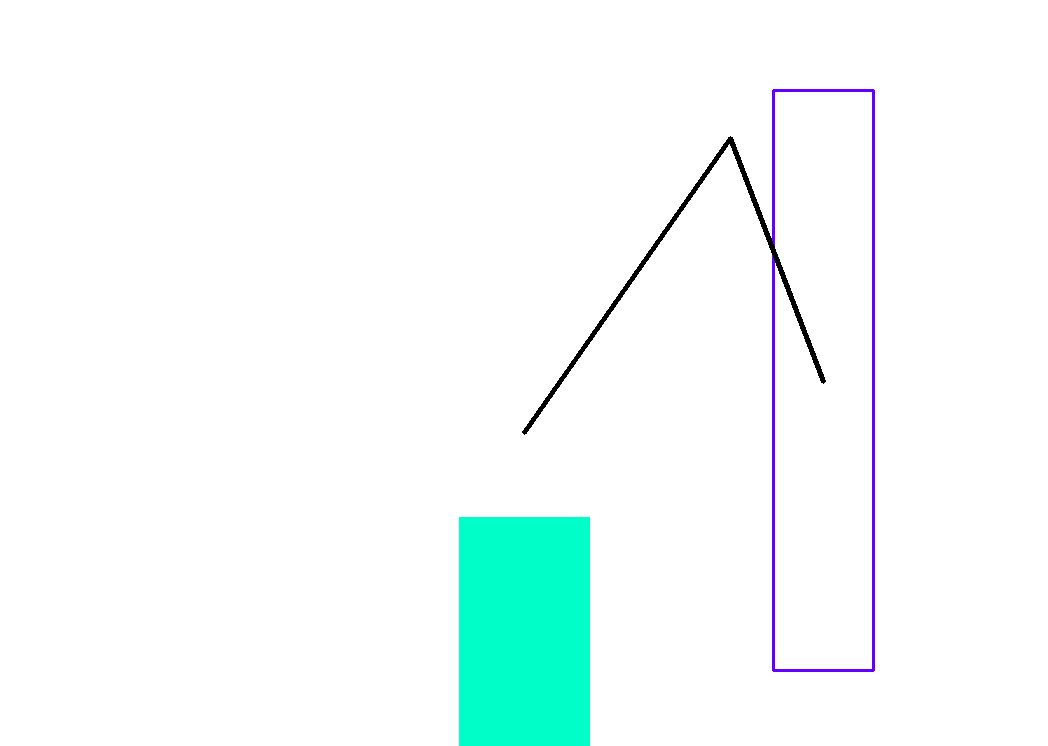
\includegraphics[width=60mm]{img/XYA-objectsize.png}}
		\caption{Objekt 100x580} \label{OBRAZOK 5.1.2.1} 
	\end{subfigure}
	\begin{subfigure}{0.4\textwidth}
		\centering
		\fbox{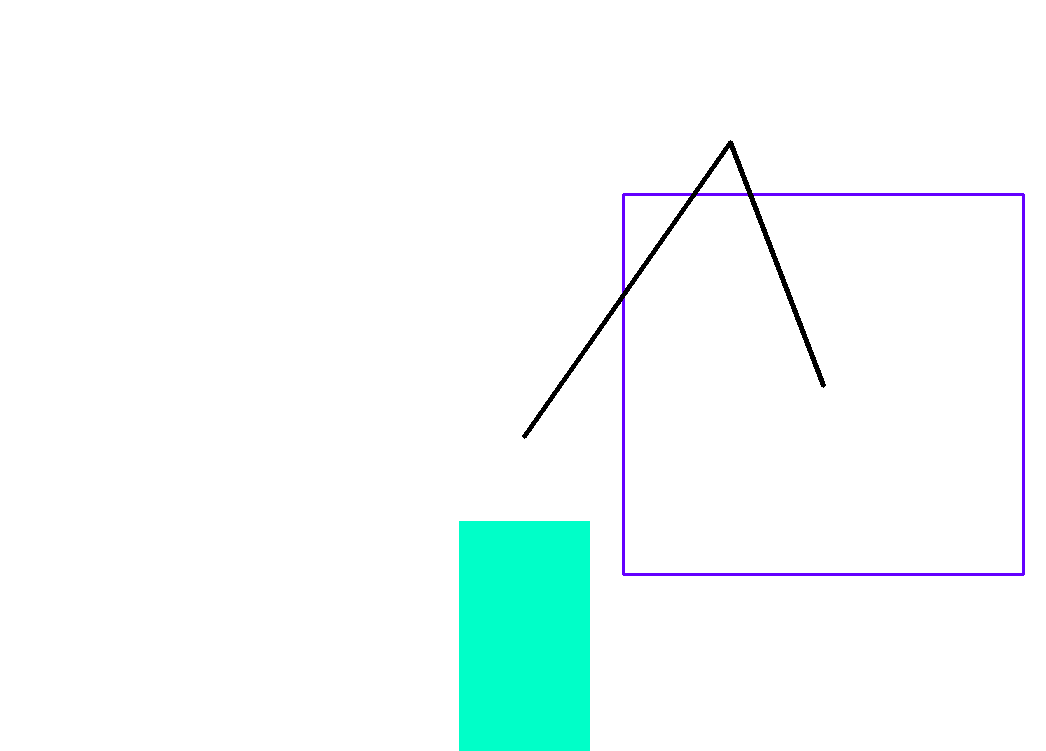
\includegraphics[width=60mm]{img/XYA-objectsize2.png}}
		\caption{Objekt 400x380} \label{OBRAZOK 5.1.2.2}
	\end{subfigure}
\caption{Maximálne rozmery objektu}
\label{OBRAZOK 5.1.2} 
\end{figure} 

Ďalším faktorom ovplyvňujúcim výber vhodného algoritmu je čas výpočtu. Priemerný čas výpočtu je $ 0,72 s$ so smerodajnou odchýlkou $ 1,4 s$.  Keďže čas výpočtu so zväčšujúcimi sa rozmermi objektu výrazne narastá rozhodli sme sa pre podobný spôsob interpretácie dát ako pri hodnotení úspešnosti dosiahnutia cieľa. Na obrázku \ref{OBRAZOK 5.1.3} môžeme vidieť graf priemerných časov pre jednotlivé rozmery objektu. Pri výpočte algoritmu sme si ako jendu z ukončovacích  podmienok nastavili aj maximálny čas výpočtu, ktorý bol pre všetky behy nastavený na 20 sekúnd. Škála nám teda zobrazuje rozsah časov od 0 po 20 sekúnd. 

\begin{figure}[h!]
	\centering
	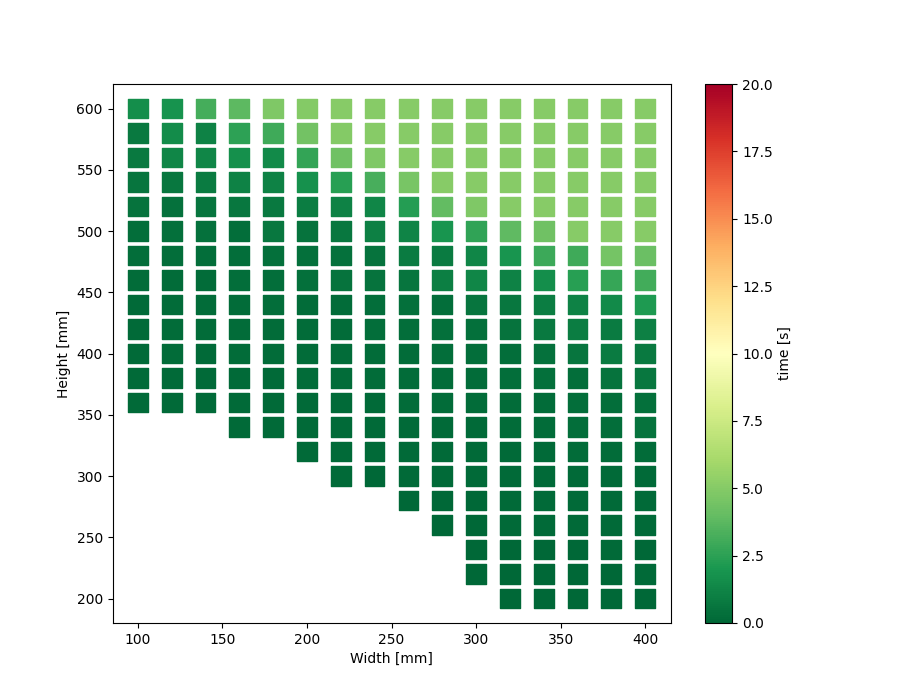
\includegraphics[width=140mm]{img/XYA-time.png}
	\caption{Kartézsky priestor (RRT) - čas} \label{OBRAZOK 5.1.3} 
\end{figure} 

Ako môžeme z grafu vidieť priemerný čas pre rozmery, pri ktorých bol algoritmus schopný nájsť riešenie sa pohybuje v časoch pod 1 sekundu. V prípade  väčších rozmeroch kde už úspešnosť klesá, resp. je nulová časy dosahujú priemernú hodnotu okolo 7 sekúnd.

Z hľadiska kvality trajektórie nám vyšla priemerná hodnota pomeru najkratšej cesty a nami nájdenej cesty $ 1.43 $. Na obrázku \ref{OBRAZOK 5.1.3.1} je vidieť príklad jedného z prípadu z testovaných konfigurácií. 
\begin{figure}[h!]
	\centering
	\fbox{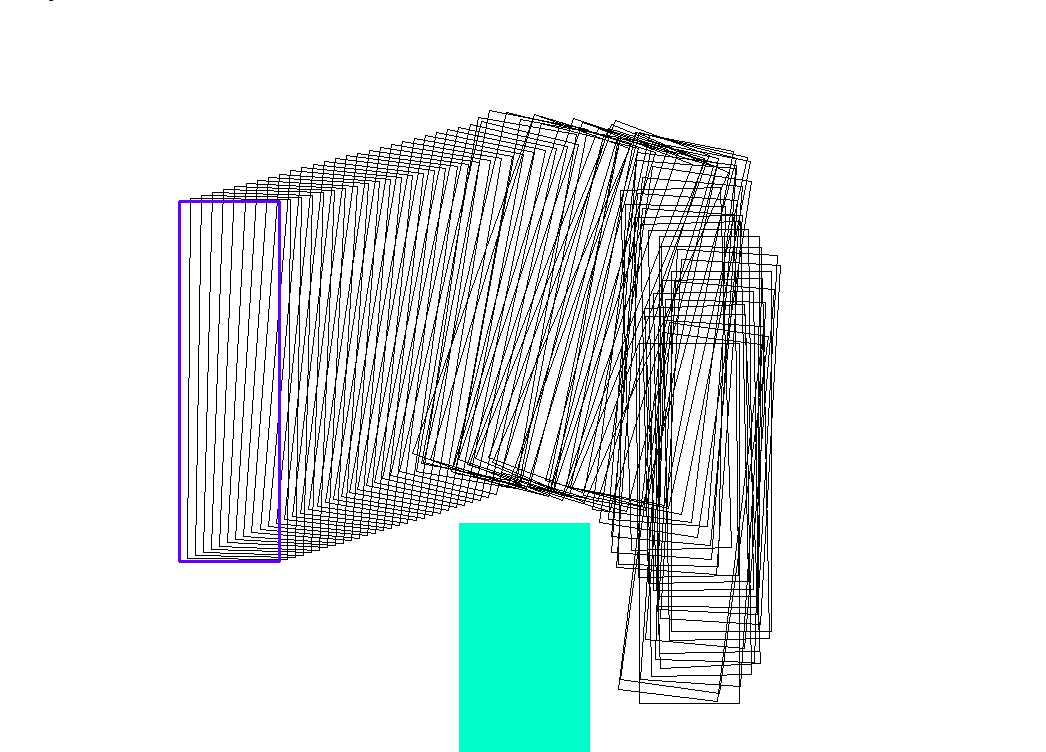
\includegraphics[width=100mm]{img/XYA-trajectory.png}}
	\caption{Trajektória - RRT } \label{OBRAZOK 5.1.3.1} 
\end{figure} 

 


\subsubsection{Kartézsky priestor - RRT*}

\begin{figure}[h]
	\centering
	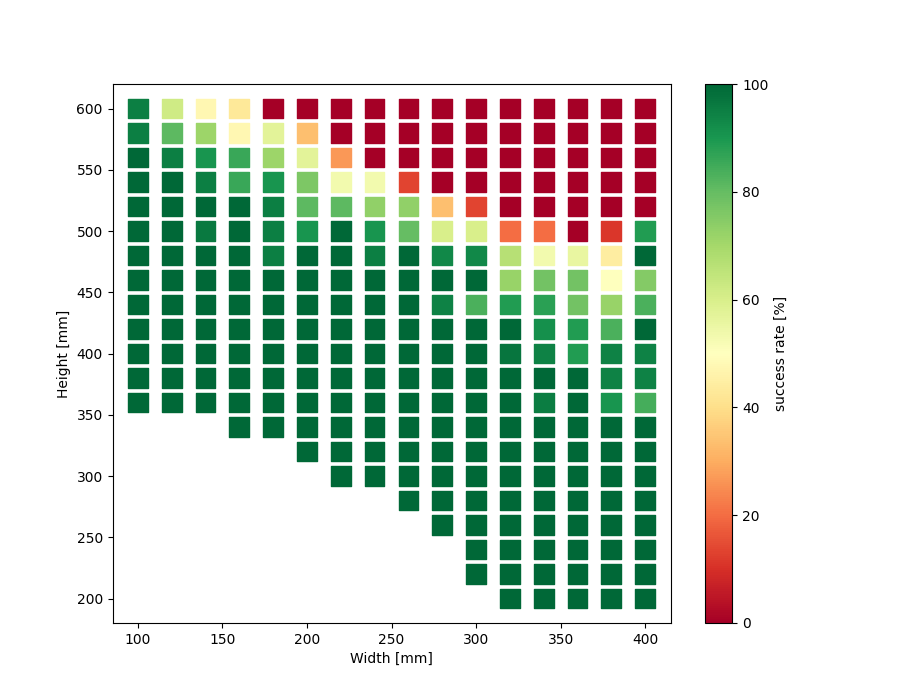
\includegraphics[width=140mm]{img/XYA-star-size.png}
	\caption{Kartézsky priestor (RRT*) - úspešnosť} \label{OBRAZOK 5.1.4} 
\end{figure} 

\begin{figure}[h]
	\centering
	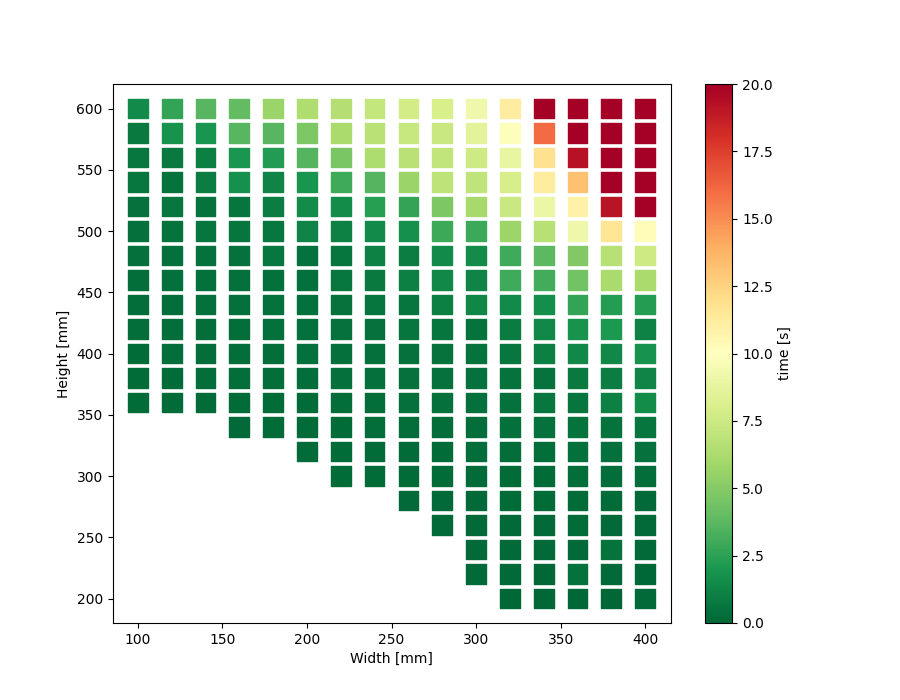
\includegraphics[width=140mm]{img/XYA-star-time.png}
	\caption{Kartézsky priestor (RRT*) - čas} \label{OBRAZOK 5.1.5} 
\end{figure} 

\subsubsection{Kĺbový priestor}

\begin{figure}[h]
	\centering
	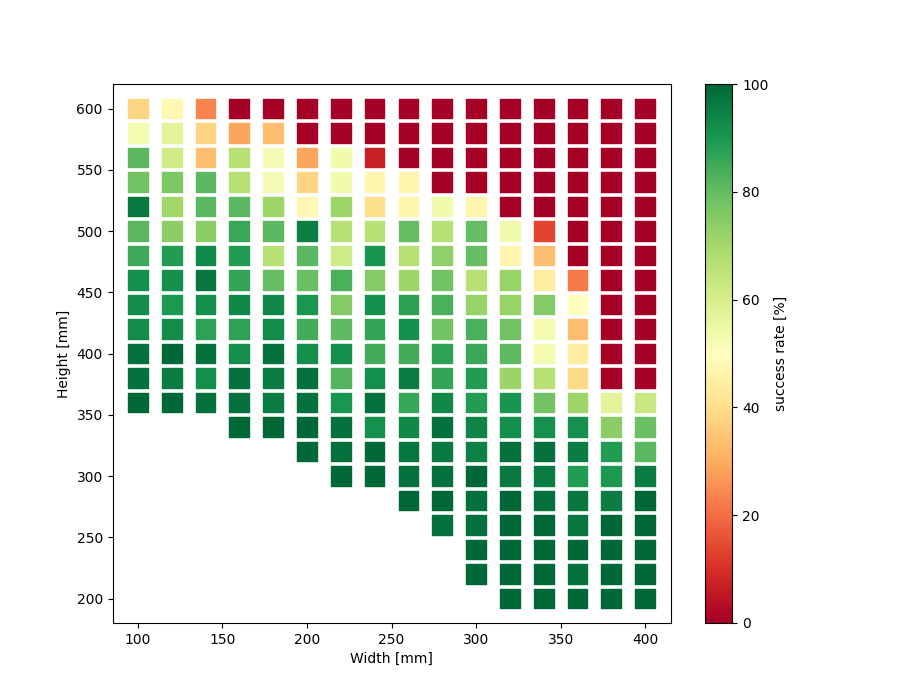
\includegraphics[width=140mm]{img/3Q-size.png}
	\caption{Kĺbový priestor (RRT) - úspešnosť} \label{OBRAZOK 5.1.7} 
\end{figure} 

\begin{figure}[h]
	\centering
	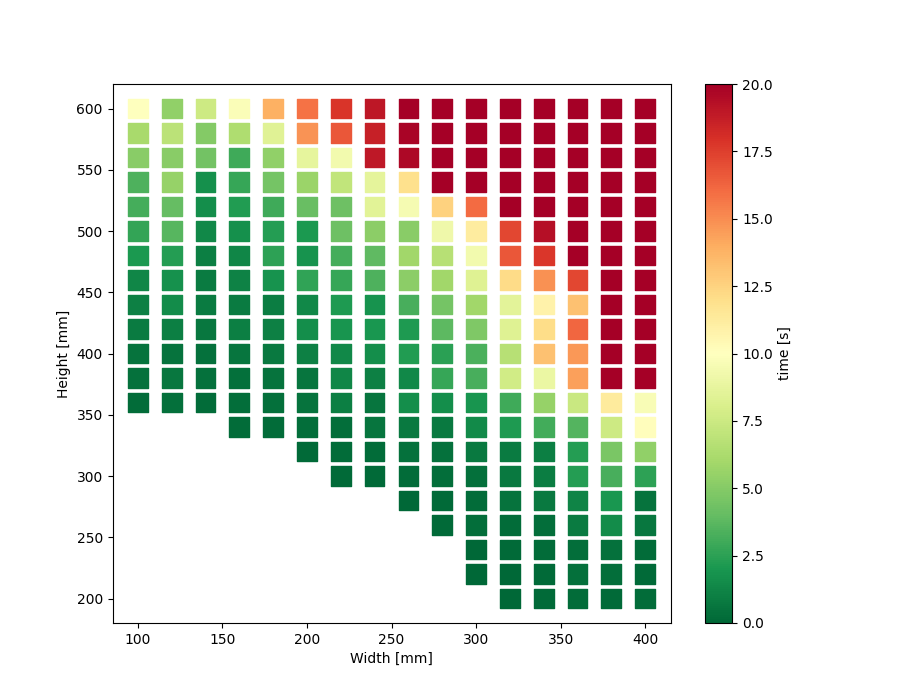
\includegraphics[width=140mm]{img/3Q-time.png}
	\caption{Kĺbový priestor (RRT) - čas} \label{OBRAZOK 5.1.8} 
\end{figure} 

\subsection{2 stupne voľnosti}
\label{kap:5.2}

\subsubsection{Bez predrotácie}


\subsubsection{Predrotácia}
\begin{figure}[h]
	\centering
	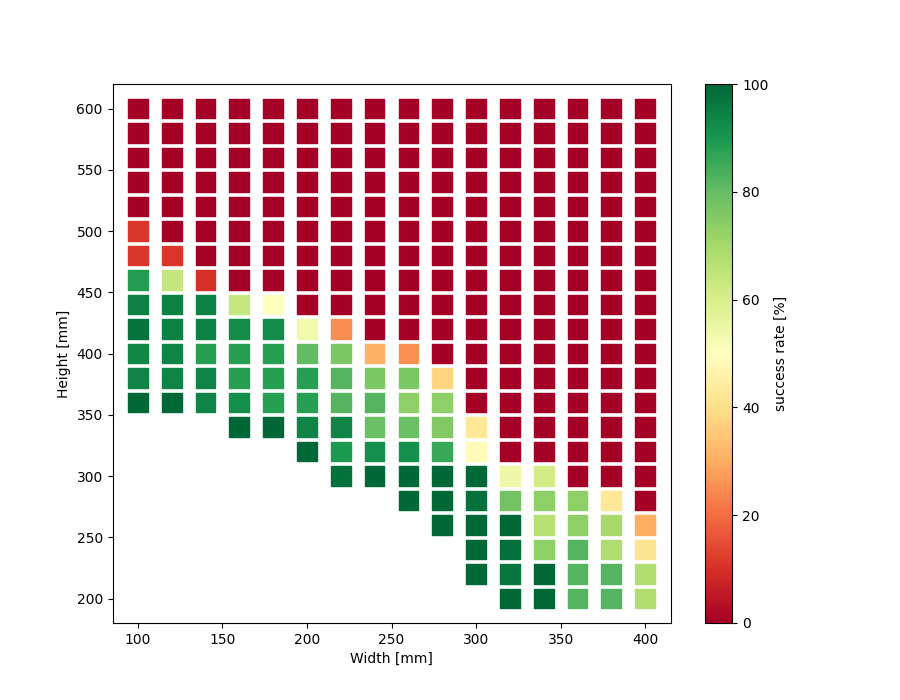
\includegraphics[width=140mm]{img/2Q-size.png}
	\caption{RRT s predrotáciou - úspešnosť} \label{OBRAZOK 5.2.1} 
\end{figure} 

\begin{figure}[h]
	\centering
	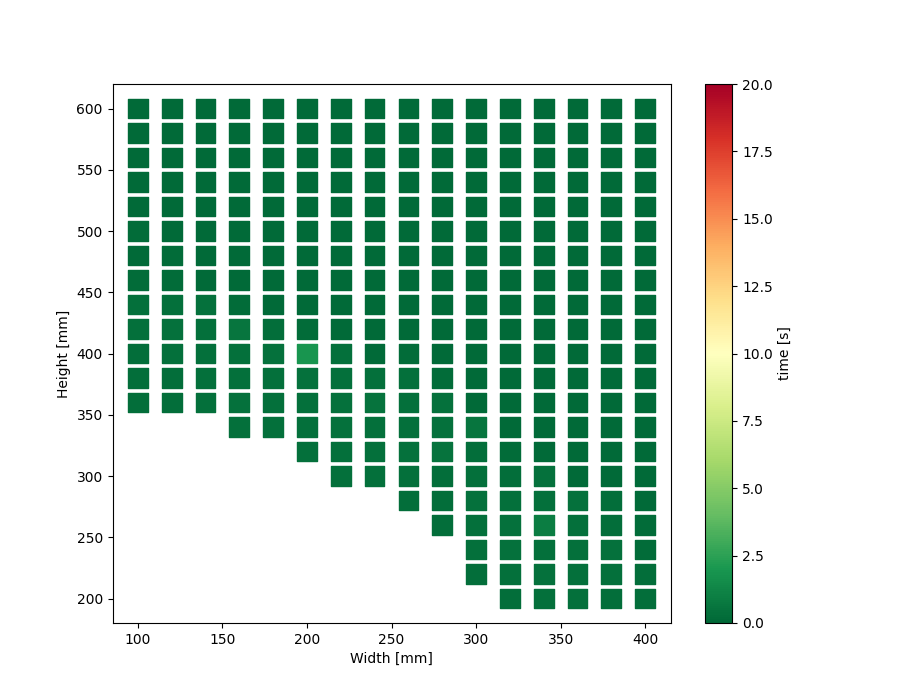
\includegraphics[width=140mm]{img/2Q-time.png}
	\caption{RRT s predrotáciou- čas} \label{OBRAZOK 5.2.2} 
\end{figure} 

\subsection{Typy objektov}
\label{kap:5.3}
- experiment s 5 typmi objektov v krabici

